\documentclass[11pt]{article}

\usepackage{nmrdoc}
\usepackage{siunitx}
\usepackage{bm}
\usepackage{tikz}

\sisetup{per-mode=symbol}
\DeclareSIUnit{\angstrom}{\text{\AA}}

\newcommand{\code}[1]{\texttt{#1}}
\setlength{\parindent}{0pt}
\setlength{\parskip}{0.42em}
\emergencystretch=2em

\begin{document}
\NmrTitle{Numerical Addendum: RingSusceptibility Calculator}

The calculator is a cutoff sum of closed-form ring kernels. The numerical
objects are the shared SVD ring geometry, the ring-centre spatial query and
filters that decide which pairs enter the sum, the McConnell form tensor with
the bond axis replaced by the ring normal, and the shared \(T_0/T_1/T_2\)
projection. The listings below are distilled from the source: loops and
bookkeeping are trimmed, but the constants, guards, inequalities, tensor
entries, and output shape are the implementation's.

\section{Ring sources and candidates}

\code{conf.ring\_geometries} gives the calculator one source geometry per
aromatic ring. Each entry carries a centre \(\bm c\), a unit normal
\(\hat{\bm n}\), a mean radius \(R\), and the ordered vertices. The centre is
the mean of the vertex coordinates. The normal is the least-variance direction
of the mean-centred vertex cloud, with its sign fixed by the first two ordered
edges. The radius is the mean centre-to-vertex distance. The full SVD plane-fit
treatment is in the Haigh--Mallion numerical addendum; this calculator consumes
only the fitted centre, normal, and mean radius.

\begin{codebox}
geo.center = mean(geo.vertices);

Eigen::MatrixXd coords(geo.vertices.size(), 3);
for (size_t i = 0; i < geo.vertices.size(); ++i)
    coords.row(i) = (geo.vertices[i] - geo.center).transpose();

Eigen::JacobiSVD<Eigen::MatrixXd> svd(coords, Eigen::ComputeFullV);
geo.normal = svd.matrixV().col(2);       // least spread

Vec3 e1 = geo.vertices[1] - geo.vertices[0];
Vec3 e2 = geo.vertices[2] - geo.vertices[0];
if (geo.normal.dot(e1.cross(e2)) < 0) geo.normal = -geo.normal;

geo.radius = mean(norm(vertex - geo.center));
\end{codebox}

For each atom, the candidate set comes from the nanoflann tree over ring
centres. The query point is the atom position and the radius is
\code{ring\_current\_spatial\_cutoff}, \(\SI{15.0}{\angstrom}\) in the shared
TOML file. The radius query decides only which ring indices are returned. A
ring not returned by the query never reaches the kernel helper; a returned ring
can still be omitted by the filters below.

\begin{codebox}
auto nearby_rings =
    spatial.RingsWithinRadius(atom_pos,
        cfg("ring_current_spatial_cutoff"));       // 15.0 A

for (size_t ri : nearby_rings) {
    const RingGeometry& geom = conf.ring_geometries[ri];
    RingChiKernelResult kernel =
        ComputeRingChiKernel(atom_pos, geom.center, geom.normal);
    ...
}
\end{codebox}

\section{One ring kernel}

For an atom at \(\bm r_i\), the helper forms
\(\bm x=\bm r_i-\bm c\), the displacement from ring centre to atom. Its length
is \(r=|\bm x|\), and \(\hat{\bm d}=\bm x/r\) is the unit centre-to-atom
direction. The angle used by the kernel enters only through
\[
  u=\cos\theta_{\mathrm{k}}=\hat{\bm d}\cdot\hat{\bm n}.
\]
If \(r<\SI{0.1}{\angstrom}\), the \code{singularity\_guard\_distance}, the
helper returns the zero-initialized result. In that return path the stored
distance remains zero, so the later distance filter rejects the candidate
instead of recording a zero-valued neighbour.

\begin{codebox}
Vec3 x = atom_pos - ring_center;          // center -> atom
double r = x.norm();
if (r < cfg("singularity_guard_distance")) return result;

result.distance = r;
double r3 = r * r * r;
Vec3 d_hat = x / r;
double u = d_hat.dot(ring_normal);        // cos(theta_k)

result.scalar_kernel = (3.0 * u * u - 1.0) / r3;
\end{codebox}

The formula is the McConnell bond-anisotropy kernel with the bond axis
\(\hat{\bm b}\) replaced by the ring normal \(\hat{\bm n}\). Under the
substitution
\[
  \hat{\bm b}\mapsto\hat{\bm n},\qquad
  c=\hat{\bm d}\cdot\hat{\bm b}\mapsto
  u=\hat{\bm d}\cdot\hat{\bm n},
\]
the ring helper has the same scalar \(f=(3u^2-1)/r^3\), the same dipolar helper
\[
  K_{ab}=\frac{3\hat d_a\hat d_b-\delta_{ab}}{r^3},
\]
and the same three-term tensor structure:
\[
  M_{ab} =
  \frac{
     9u\,\hat d_a\hat n_b
    -3\hat n_a\hat n_b
    -\left(3\hat d_a\hat d_b-\delta_{ab}\right)}
  {r^3}.
\]
The helper stores \(K\), but RingSusceptibility does not write it to any feature
field. The per-ring neighbour fields store \(\bm M\), with units
\(\si{\angstrom^{-3}}\). This class does not multiply by a ring-current
intensity, a Johnson--Bovey lobe offset, a susceptibility scale, or a
ring-type weight.

\begin{codebox}
for (int a = 0; a < 3; ++a)
    for (int b = 0; b < 3; ++b)
        result.dipolar_kernel(a,b) =
            (3.0*d_hat(a)*d_hat(b) - (a == b ? 1.0 : 0.0)) / r3;

for (int a = 0; a < 3; ++a) {
    for (int b = 0; b < 3; ++b) {
        double Iab = (a == b ? 1.0 : 0.0);
        result.full_tensor_over_r3(a,b) =
            (9.0*u*d_hat(a)*ring_normal(b)
             - 3.0*ring_normal(a)*ring_normal(b)
             - (3.0*d_hat(a)*d_hat(b) - Iab)) / r3;
    }
}
\end{codebox}

The three terms determine which tensor channels can be populated. The trace of
the first term is \(9u^2\), the trace of the second is \(-3\), and the
third term is traceless, so
\[
  T_0(\bm M)=\frac{1}{3}\operatorname{tr}\bm M
            =\frac{3u^2-1}{r^3}=f .
\]
The antisymmetric part can only come from
\(9u\,\hat{\bm d}\otimes\hat{\bm n}\). It is proportional to
\(u(\hat{\bm d}\otimes\hat{\bm n}
-\hat{\bm n}\otimes\hat{\bm d})\), so it vanishes when \(\hat{\bm d}\) is
parallel or antiparallel to \(\hat{\bm n}\) (the atom on either end of the ring
axis, \(u=\pm1\)) and when \(u=0\) (the atom in the ring plane). Away from those
geometries it can survive as \(T_1\). The symmetric traceless remainder fills
\(T_2\).

\section{Ring-frame coordinates}

The shared neighbour record also carries the accepted atom in a cylindrical
frame tied to the same fitted ring geometry. When RingSusceptibility creates
the record, the axial coordinate is
\[
  z=\bm x\cdot\hat{\bm n},
\]
and the in-plane radial vector is
\(\bm x_\perp=\bm x-z\hat{\bm n}\), with \(\rho=|\bm x_\perp|\). Since
\(\hat{\bm n}\) is unit length, \(r^2=z^2+\rho^2\). The kernel angle above uses
the signed cosine \(u=z/r\). The stored polar angle is different:
\[
  \theta_{\mathrm{store}}=\operatorname{atan2}(\rho,|z|),
  \qquad
  \cos\theta_{\mathrm{store}}=|z|/r=|u|.
\]
The absolute value folds the two faces of the ring together. The sign of \(z\)
still records which face the atom lies on, with the ring normal's code-defined
orientation, but \(\theta_{\mathrm{store}}\) alone cannot distinguish
\((z,\rho)\) from \((-z,\rho)\). Its range is \([0,\pi/2]\), from on-axis to
in-plane.

\begin{codebox}
Vec3 atom_offset = atom_pos - geom.center;
double z = atom_offset.dot(geom.normal);
Vec3 d_plane = atom_offset - z * geom.normal;
double rho = d_plane.norm();
double theta = std::atan2(rho, std::abs(z));

new_neighbour.z = z;
new_neighbour.rho = rho;
new_neighbour.theta = theta;
\end{codebox}

\begin{figure}[ht]
\centering
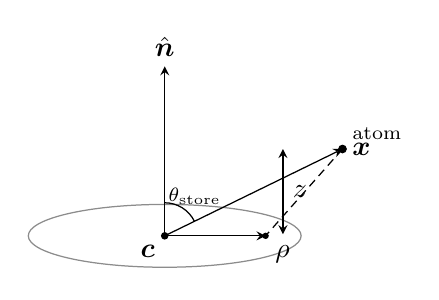
\begin{tikzpicture}[scale=1.05,line width=0.45pt,>=stealth]
  \coordinate (C) at (0,0);
  \coordinate (A) at (2.15,1.05);
  \coordinate (P) at (1.22,0.00);
  \draw[black!45] (C) ellipse (1.65 and 0.38);
  \draw[->] (C) -- (0,2.05) node[above] {\(\hat{\bm n}\)};
  \draw[->] (C) -- (A) node[right] {\(\bm x\)};
  \draw[densely dashed] (A) -- (P);
  \draw[->] (C) -- (P) node[below right] {\(\rho\)};
  \draw[<->] (1.43,0.02) -- (1.43,1.05) node[midway,right] {\(z\)};
  \draw (0,0.40) arc[start angle=90,end angle=26,radius=0.40];
  \node at (0.36,0.48) {\scriptsize \(\theta_{\mathrm{store}}\)};
  \fill (C) circle (1.3pt) node[below left] {\(\bm c\)};
  \fill (A) circle (1.5pt) node[above right] {\scriptsize atom};
  \fill (P) circle (1.1pt);
\end{tikzpicture}
\caption{The neighbour coordinates split the centre-to-atom offset into axial
\(z\) and radial \(\rho\). The stored angle uses \(|z|\), so points on the two
faces have the same \(\theta_{\mathrm{store}}\) when their \(|z|\) and
\(\rho\) match.}
\end{figure}

\section{Filters and omissions}

The per-atom path calls the kernel helper before it applies the filter set, but
a rejected pair changes no accumulators. It does not create or update a
ring-neighbour record, does not add \(\chi_{\mathrm{scalar}}\), and does not
add \(\bm M\) to the atom total.

\begin{codebox}
filters.Add(std::make_unique<MinDistanceFilter>());
filters.Add(std::make_unique<DipolarNearFieldFilter>());
filters.Add(std::make_unique<RingBondedExclusionFilter>(protein));

ctx.distance = kernel.distance;
ctx.source_extent = 2.0 * geom.radius;       // ring diameter
ctx.atom_index = ai;
ctx.source_ring_index = ri;
if (!filters.AcceptAll(ctx)) continue;
\end{codebox}

\code{MinDistanceFilter} requires
\[
  r \ge \code{singularity\_guard\_distance}
    = \SI{0.1}{\angstrom}.
\]
For a closer point the helper has already returned a zero tensor and left
\code{kernel.distance} at zero; the filter turns that guarded helper result
into an omitted pair. The omitted term is not replaced by a clamped
\(r=\SI{0.1}{\angstrom}\) contribution.

\code{DipolarNearFieldFilter} uses the ring diameter \(2R\) as
\code{source\_extent}. With the configured ratio \(0.5\), the atom path
accepts only
\[
  r > 0.5(2R)=R .
\]
This is a centre-distance test against the mean-radius sphere. It is not a
point-in-polygon test on the ring plane, and it does not use \(\rho\). A
candidate at or inside that boundary leaves the sum.

\code{RingBondedExclusionFilter} is topological. At construction it walks each
ring vertex and all bonds incident on that vertex, then stores a per-ring set
containing the vertices and their covalently bonded neighbours. If the target
atom is in the set for the source ring, the pair is omitted even when the
distance filters would accept it.

The grid-sampling path uses the same kernel and the same configured distances,
but not the atom filter set. It loops over all aromatic rings, skips
\(r<\SI{0.1}{\angstrom}\), skips \(r<R\), and skips
\(r>\SI{15.0}{\angstrom}\). It therefore keeps equality at the near-field
boundary \(r=R\), while the per-atom filter path rejects equality. It has no
bonded exclusion because a free grid point has no atom index or covalent
topology.

\begin{codebox}
double r = (point - geom.center).norm();
if (r < cfg("singularity_guard_distance")) continue;
if (r < geom.radius) continue;
if (r > cfg("ring_current_spatial_cutoff")) continue;

auto kernel = ComputeRingChiKernel(point, geom.center, geom.normal);
M_total += kernel.full_tensor_over_r3;
\end{codebox}

\code{near\_zero\_vector\_norm\_threshold} is present in the shared parameter
file with value \(10^{-10}\), but this calculator does not read it.

\section{Accumulation and projection}

Accepted per-ring tensors are added as raw \(3\times3\) matrices:
\[
  \bm M_i=\sum_{R\in\mathcal A_i}\bm M^{(iR)} .
\]
Both the per-ring neighbour tensor and the per-atom total go directly to
\code{SphericalTensor::Decompose}. There is no symmetrization
\(\frac12(M+M^{\mathsf T})\) and no trace removal before the call.

\begin{codebox}
neighbour->chi_tensor = kernel.full_tensor_over_r3;
neighbour->chi_spherical =
    SphericalTensor::Decompose(kernel.full_tensor_over_r3);
neighbour->chi_scalar = kernel.scalar_kernel;

M_total += kernel.full_tensor_over_r3;

atom.ringchi_shielding_contribution =
    SphericalTensor::Decompose(M_total);
\end{codebox}

This is the full-tensor path from the McConnell calculator, with no category
\(T_2\) path beside it. McConnell reports some bond-category tensors after
symmetrizing and subtracting the trace, and also reports the raw full
\(\bm M_{\mathrm{total}}\) decomposition. RingSusceptibility uses only the raw
full decomposition. The consequence is that the antisymmetric part of the first
dyad is retained as nonzero \(T_1\) whenever the accepted geometry leaves one.

The shared projection is closed-form arithmetic on a \(3\times3\) tensor
\(\bm X\). The trace gives \(T_0\), the antisymmetric part gives the Cartesian
Levi-Civita dual \(T_1\), and the symmetric traceless part gives the five
stored \(T_2\) numbers.

\begin{codebox}
st.T0 = sigma.trace() / 3.0;

st.T1[0] = 0.5*(sigma(1,2) - sigma(2,1));
st.T1[1] = 0.5*(sigma(2,0) - sigma(0,2));
st.T1[2] = 0.5*(sigma(0,1) - sigma(1,0));

double Sxx = sigma(0,0) - st.T0;
double Syy = sigma(1,1) - st.T0;
double Szz = sigma(2,2) - st.T0;
double Sxy = 0.5*(sigma(0,1) + sigma(1,0));
double Sxz = 0.5*(sigma(0,2) + sigma(2,0));
double Syz = 0.5*(sigma(1,2) + sigma(2,1));

st.T2[0] = std::sqrt(2.0) * Sxy;
st.T2[1] = std::sqrt(2.0) * Syz;
st.T2[2] = std::sqrt(3.0/2.0) * Szz;
st.T2[3] = std::sqrt(2.0) * Sxz;
st.T2[4] = (Sxx - Syy) / std::sqrt(2.0);
\end{codebox}

The \(T_2\) constants make the five-number packing isometric. An off-diagonal
entry such as \(S_{xy}\) appears twice in the symmetric matrix, as \(S_{xy}\)
and \(S_{yx}\), so it contributes \(2S_{xy}^2\) to the Frobenius sum. The
stored \(\sqrt2\,S_{xy}\) squares to the same amount. The diagonal entries have
only two degrees of freedom after \(S_{xx}+S_{yy}+S_{zz}=0\); the
\(\sqrt{3/2}\,S_{zz}\) and \((S_{xx}-S_{yy})/\sqrt2\) entries carry those two
degrees so their squares add back to the diagonal Frobenius contribution.

\code{ringchi\_shielding.npy} has shape \(N\times9\), one row per atom, in the
shared packed order
\[
  [T_0,T_{1x},T_{1y},T_{1z},
    T_{2,-2},T_{2,-1},T_{2,0},T_{2,+1},T_{2,+2}] .
\]

\section{Glossary}

\textbf{Dyadic product.} A grid where one vector labels the rows and the other
labels the columns, every cell holding the product of its two labels. In this
calculator,
\(\hat{\bm d}\otimes\hat{\bm n}\) has entry \(\hat d_a\hat n_b\), so swapping
the indices can change the value. Formally,
\((\bm p\otimes\bm q)_{ab}=p_aq_b\).

\textbf{Dipolar helper \(K\).} The bar-magnet field shape laid along the
centre-to-atom line --- strongest and signed down that axis, weaker and reversed
to the side (a symmetric traceless tensor), assembled before the full ring
tensor but not emitted.
It has eigenvalue \(+2/r^3\) along \(\hat{\bm d}\) and \(-1/r^3\) in each
transverse direction. Formally,
\(K_{ab}=(3\hat d_a\hat d_b-\delta_{ab})/r^3\).

\textbf{Near-field exclusion.} A bubble drawn around the ring, sized to the real
loop the point kernel stands in for (a centre-distance exclusion sphere whose
radius is the mean ring radius). For a ring with mean
radius \(R\), it omits the candidate unless \(r>R\). Formally, the filter is
\(r>\rho_{\mathrm{nf}}E\), with \(E=2R\) and
\(\rho_{\mathrm{nf}}=0.5\).

\textbf{Spherical tensor split.} A \(3\times3\) tensor holds three kinds of
content that rotate without mixing --- an orientation-free size (the scalar
trace, \(T_0\)), an axial twist from its antisymmetric part (the three \(T_1\)
components), and a five-number traceless shape for the rest of the
direction-dependence (the five \(T_2\) components).
RingSusceptibility feeds the raw
asymmetric McConnell form tensor into that split, so all nine stored numbers can
be populated. Formally, it is the closed-form split of a \(3\times3\) tensor's
nine components into dimensions \(1+3+5\), with the \(T_2\)
basis normalized to preserve the Frobenius norm.

\end{document}
